Development of MIDAS\footnote{The name MIDAS: Modeling Infrastructure for
Debugging and Simulation was a working backronym conceived of by Jack Koenig in
2015. Only later did we learn the proposed successor to RAMP Gold was also to
be named Midas (A tool to automatically transform a design into [RAMP]gold).
The name stuck.} began in 2016 with the amalgamation of the Chisel3 port of
Strober and a demo of an earlier version of the generator presented here.
Strober is not subsumed by MIDAS.  Rather, Strober uses MIDAS to generator a
simulator that can then be used to collect target state.  As a final
introductory note, MIDAS is still very much in its infancy; many of the details
described here may, and likely will, change in the future.

\begin{figure}
	\centering
	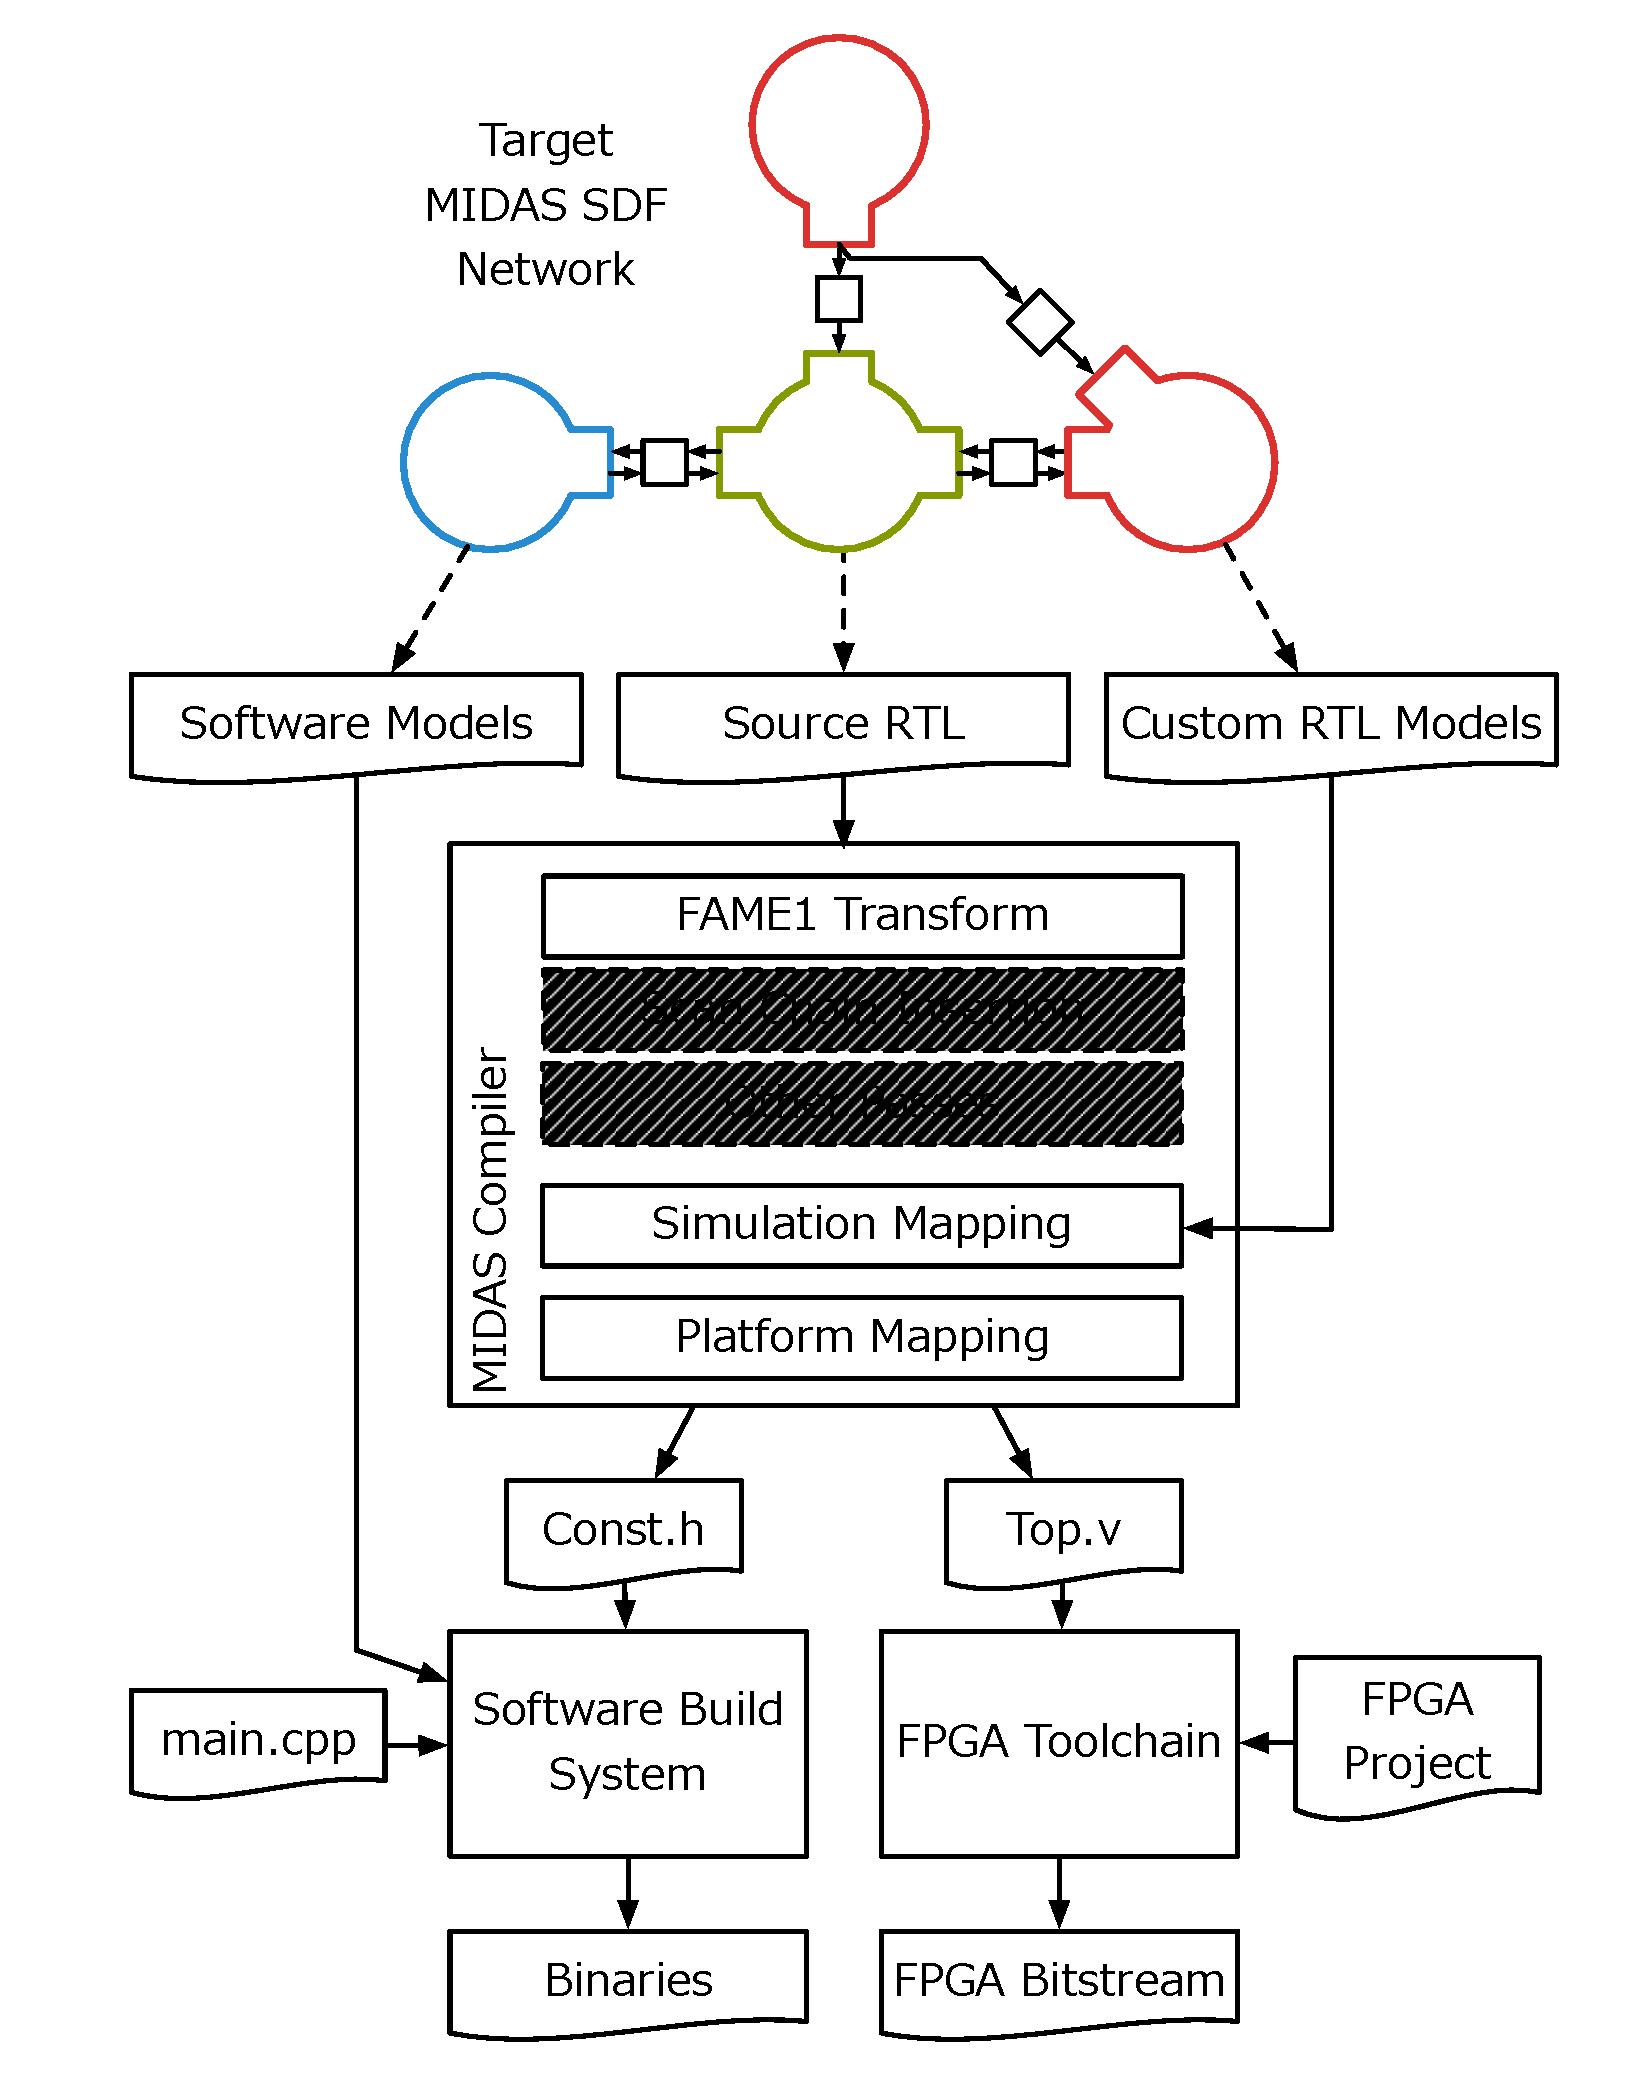
\includegraphics[width=16cm]{figures/toolchain.pdf}
    \caption{The MIDAS flow.}
	\label{fig:midas}
\end{figure}

MIDAS is a set of C++ and RTL libraries alongside a compiler. The current MIDAS
flow is shown in figure~\ref{fig:midas}. MIDAS accepts a description of target
as a synchronous dataflow (SDF)-like network of interconnected models, which
specifies how it is composed of transformed-RTL models, custom-RTL models, and
software models.

First, the MIDAS compiler automatically transforms source RTL into
host-decoupled RTL models, instrumenting them if desired. Next, it performs
\emph{simulation mapping}, during which all FPGA-hosted models are connected to
one another, and to endpoints that implement latency-insensitive communication
to models that aren't hosted locally. During this process, the compiler builds
up a memory map of all the stateful components of the simulation and ties them
together with an AXI4 bus. In \emph{platform mapping}, the simulation-mapped
design is connected to the memory and communication resources exposed by the
FPGA-host. The compiler emits a verilog file that is included in an FPGA
project and a C header that describes the simulation memory map.  With this
memory map, the simulation designer builds a main that sequences simulation by
invoking commands defined in MIDAS libraries and links in the software models
of the target.

\section{Target Specification and Simulation Abstractions}\label{sec:sdf}

In MIDAS, the target design is specified as a synchronous dataflow(SDF)-like
network of \emph{models}, connected with FIFO \emph{channels}, that carry
simulation \emph{tokens}. This is akin to model of target description used in
RAMP~\cite{ramp} and APorts~\cite{APortNetworks}). This description is sufficient
to capture the RTL behavior of the target, while still enabling a wide range of
optimizations that make FPGAs more effective accelerators for simulation. An
example MIDAS SDF shown in figure~\ref{fig:adder-example}.

\begin{figure}
	\centering
	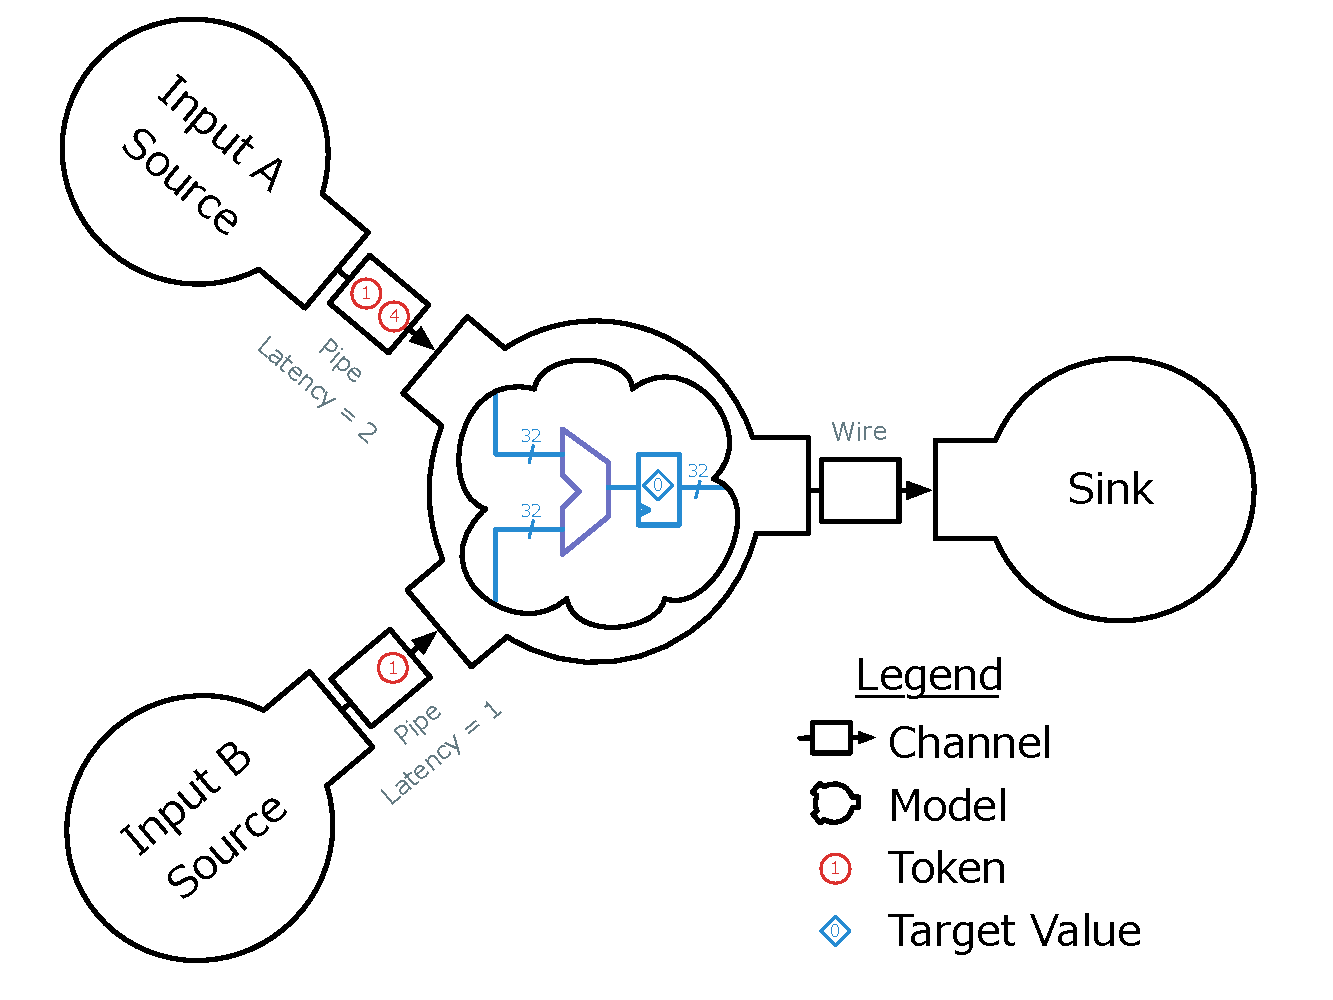
\includegraphics[width=16cm]{figures/adder-example.pdf}
    \caption{A MIDAS SDF network of a single-cycle 32-bit unsigned adder with initial tokens.}
	\label{fig:adder-example}
\end{figure}

\emph{Models} capture the behavior of a synchronous block of digital logic (an
ALU, a processor pipeline, a cache, etc...). A model advances one cycle in
target-time -- it \emph{fires} -- by dequeuing a single token from each of its
input channels, and has enqueuing a single token into each of its output
channels.  Models must dequeue from each input and into enqueue each output
exactly once before they may dequeue younger inputs tokens: they may never
``peek" ahead.

\emph{Tokens} are the basic quantum of data in the simulation. A token is
defined by a type, corresponding to the target wire that carries it, and a
value, representing the state of that wire after it has ``settled" for that
cycle.

\emph{Channels} carry tokens between models in FIFO order, and simulate the
target interconnect between those models. MIDAS has a single primitive type of
channel --  the \emph{pipe} -- which represents a pipeline with 0 more register
stages. A wire is a degenerate pipe; it has zero register stages. In MIDAS,
channels implement clock domain crossing (CDC).  Channels accomplish this by
duplicating or destroying tokens based on the relative clock frequency of the
models they connect.\footnote{The channel differs from a classical SDF channel
in two ways.  Firstly, to implement CDC in an SDF, an intermediate process
would need to be placed between two channels. Second, MIDAS channels are not
infinitely deep.  (Though, one could mimic a finite channel in an SDF with a
bidirectional pair of channels: one carrying the original tokens from source to
sink, and the second carrying credit tokens from sink to source.)} To describe
latency-insensitive interconnect in a target, MIDAS also has a
\emph{queue}-type channel. Using queue-type channels permits simulation
optimizations that would be impossible by describing the same interconnect with
some combination of pipes and models.

At time zero each of the channels is initialized with a sequence of tokens based
on the type of target interconnect they model. A pipe is initialized with tokens
equal to its latency. After initialization, target-time advances in a decoupled
fashion with models firing as they may do so legally (all of their input tokens
are available and all their output channels are not full). The
figures~\ref{fig:adder-execution}a~-~\ref{fig:adder-execution}d illustrate the
execution of the example SDF in figure~\ref{fig:adder-example} over two target
cycles.

\begin{sidewaysfigure}
    \begin{subfigure}[t]{0.45\textwidth}
	    \centering
        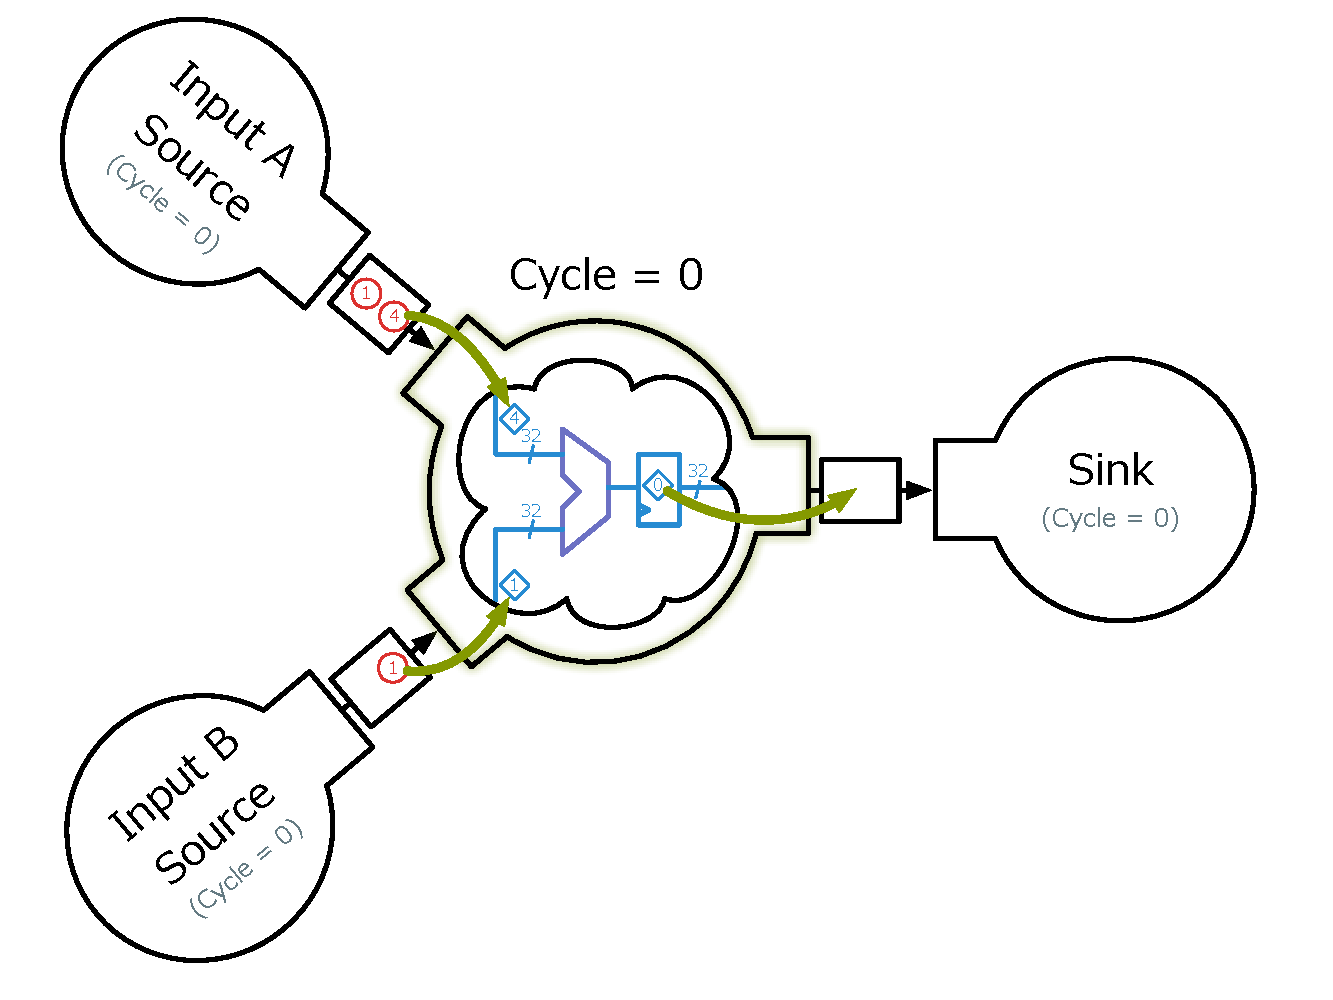
\includegraphics[width=\linewidth]{figures/adder-ex1.pdf}
        \caption{The adder model executes cycle zero, advancing ahead of the other models
        in the network.}
    \end{subfigure}
    \begin{subfigure}[t]{0.45\textwidth}
	    \centering
        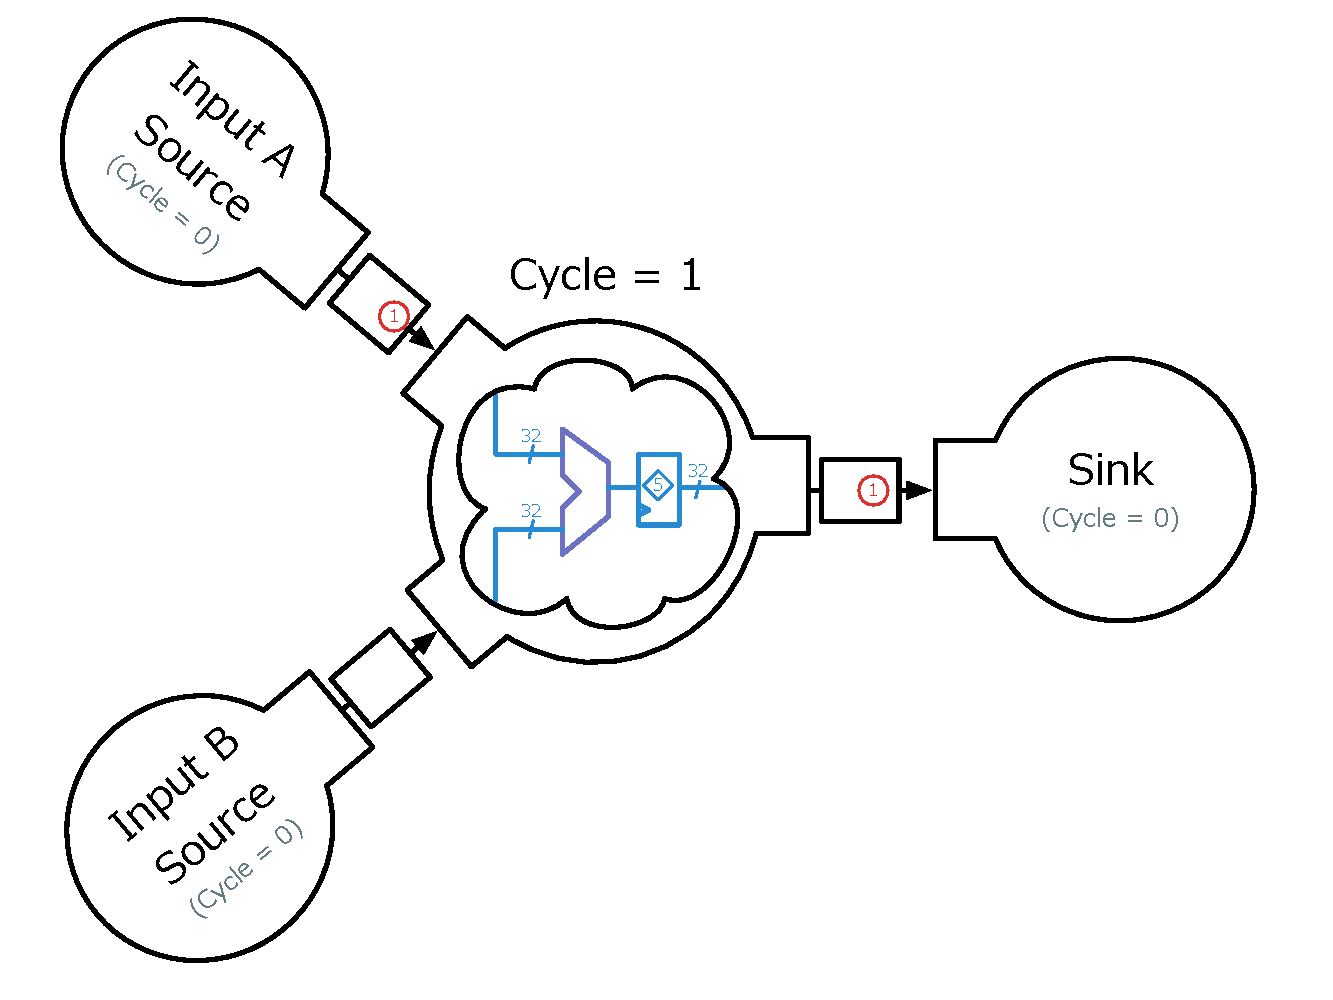
\includegraphics[width=\linewidth]{figures/adder-ex2.pdf}
        \caption{After having advanced to the next cycle, the adder model stalls as
        it cannot proceed until there is another B input token.}
    \end{subfigure}
    \begin{subfigure}[t]{0.45\textwidth}
	    \centering
        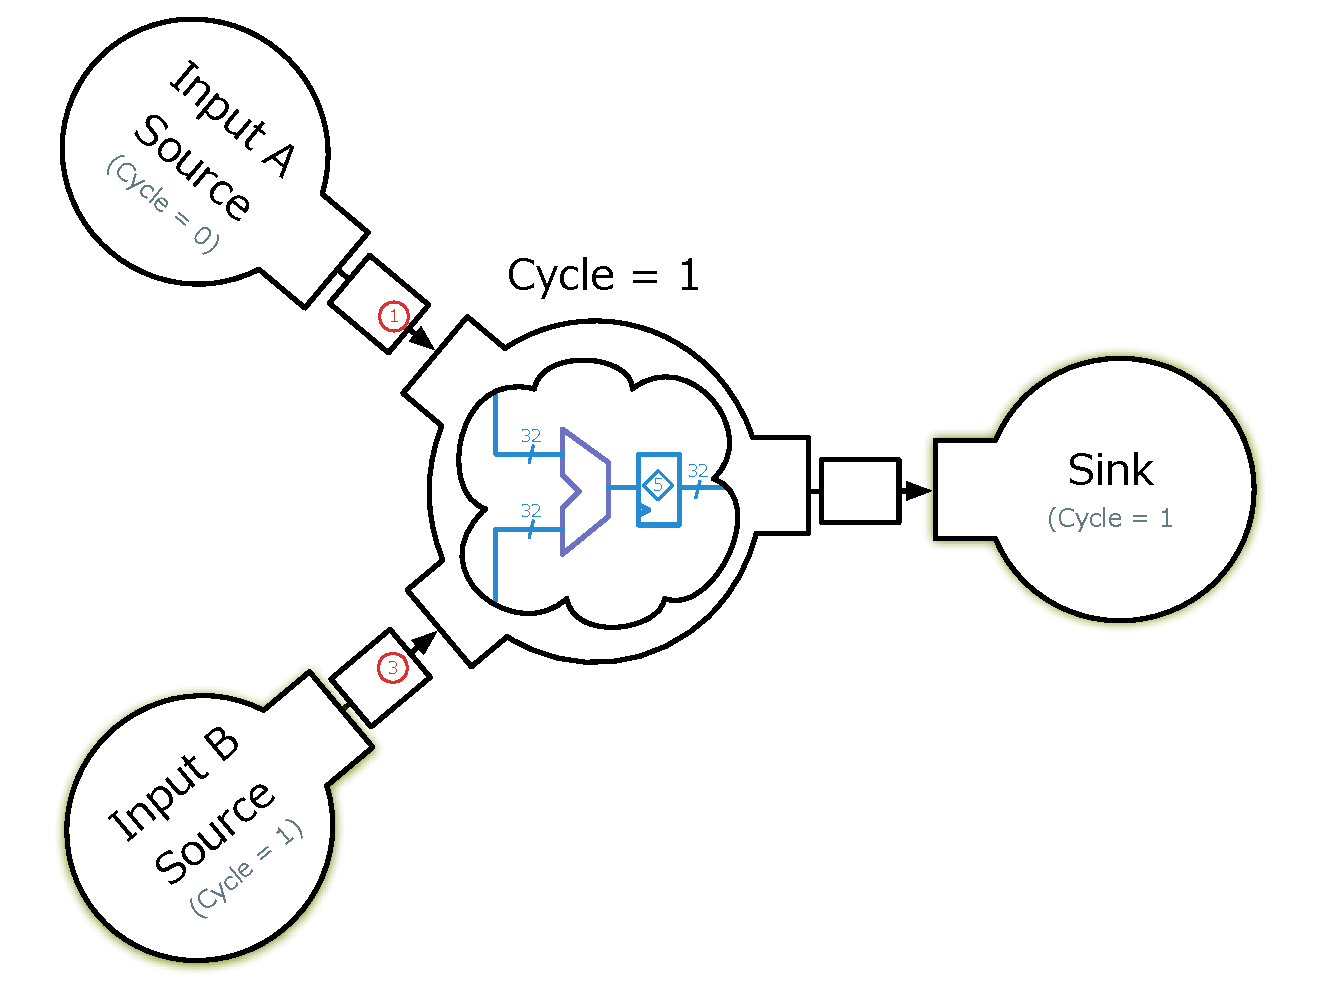
\includegraphics[width=\linewidth]{figures/adder-ex3.pdf}
        \caption{Eventually, the input B source model fires providing the needed token. The sink model may or
        may not have consumed the output in this time.}
    \end{subfigure}\hspace{0.1\linewidth}
    \begin{subfigure}[t]{0.45\textwidth}
	    \centering
        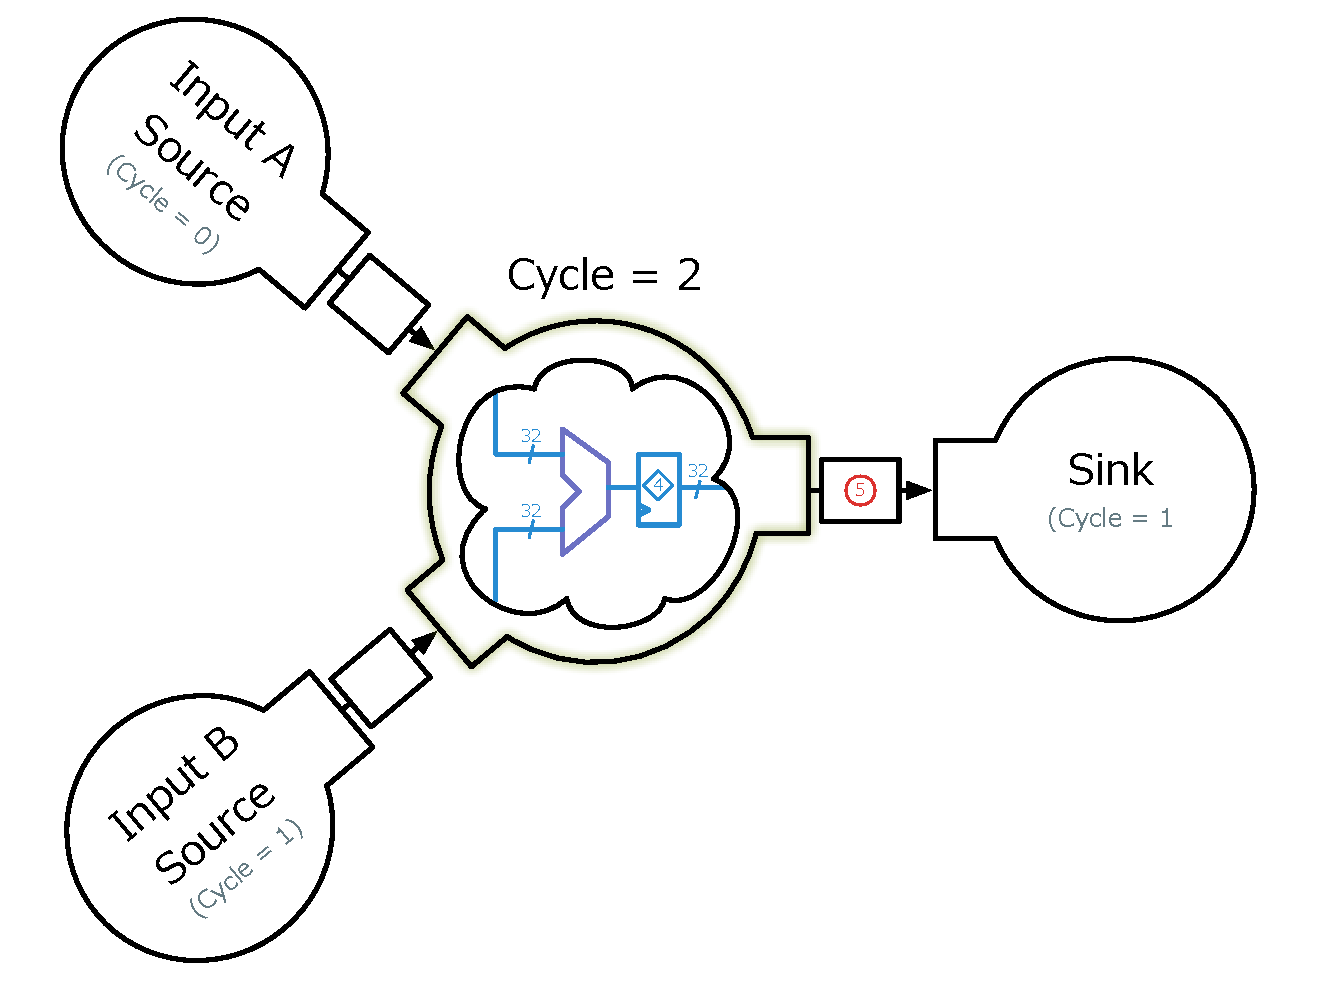
\includegraphics[width=\linewidth]{figures/adder-ex4.pdf}
        \caption{The state of the graph after the model fires a second time.}
    \end{subfigure}
    \caption{Example execution of the adder model advancing two target-cycles.}
    \label{fig:adder-execution}
\end{sidewaysfigure}

\emph{Deadlock} occurs if no model can advance (not all of its input tokens are
available or one of its output channels is full). Generally, this occurs when
the SDF network includes a cycle of wire-type channels -- it need not be a
combinational loop.  A common example of this involves decoupled source to a
model of a decoupled sink with a wire-type channels (shown in
Figure~\ref{fig:deadlock}). Judicious choice of channel type is required to
prevent this. There are two solutions to the deadlock example
in~\ref{fig:deadlock}.  Figure~\ref{fig:pipe-decoupled-example} moves the
output registers of the source into the channel, preserving the RTL behavior of
the initial SDF but requiring changes to the decoupled-source model.
Figure~\ref{fig:queue-decoupled-example} uses a queue-type channel. This
changes the RTL behavior of the target, but requires no changes to the models.
Assuming downstream models are latency insensitive this should not change the
functional behavior of the target.


\begin{figure}
    \centering
    \begin{subfigure}[t]{0.6\textwidth}
        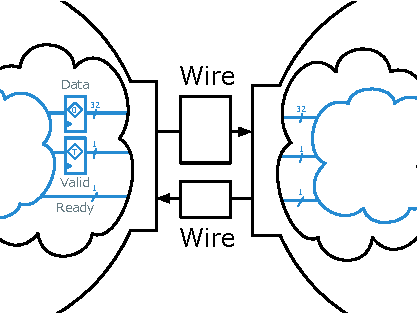
\includegraphics[width=\textwidth]{figures/deadlock.pdf}
        \caption{Using wire-type channels to implement ready-valid target interconnect in the target deadlocks the graph at time zero.}
        \label{fig:default-target}
    \end{subfigure}\vspace{0.5cm}
    \begin{subfigure}[t]{0.48\textwidth}
        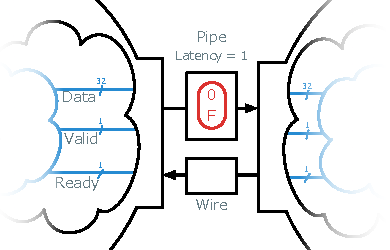
\includegraphics[width=\textwidth]{figures/pipe-decoupled-example.pdf}
        \caption{Solution A, use a pipe. Moving registers into the channel adds an initial token. While
        this graph may not deadlock, the two models can never fire concurrently
        as the decoupled sink must first fire to produce a ready token.}
        \label{fig:pipe-decoupled-example}
    \end{subfigure}\hspace{0.5cm}
    \begin{subfigure}[t]{0.48\textwidth}
        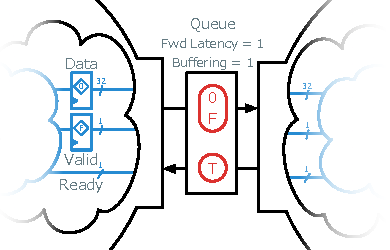
\includegraphics[width=\textwidth]{figures/queue-decoupled-example.pdf}
        \caption{Solution B, use a queue. Using a queue changes the RTL
        behavior of target -- there's extra latency moving from source to sink.
        However, in addition to requiring no changes to the models, using a queue may also
        permit both models to fire concurrently as a queue may generate
        ready tokens early if knows it will have space its buffer.}
        \label{fig:queue-decoupled-example}
    \end{subfigure}
\end{figure}

A simulator that faithfully implements an SDF network of this form decouples
target-time from host-time: it may take an arbitrary (but finite) host-time for
tokens to pass through channels, or for models to fire. (It is said to be
\emph{host-decoupled}) A model that is host-decoupled may optimized by
performing transformations maintain their token input-output behavior.

When a model is hosted on an FPGA this implies that one target-cycle may
execute over an arbitrary number of FPGA-host clock cycles.  ASIC structures
that map poorly to an FPGA when implemented directly, like CAMs and
multi-ported RAMs, can instead by simulated over multiple host-cycles with
fewer resources and greater host frequency.

To help quantify this time-area trade-off it is useful to define FPGA-cycle to
Model-Cycle Ratio~\cite{APorts}, the mean number of FPGA-cycles required to
execute a single target-cycle: $$ FMR = \frac{Cycles_{FPGA}}{Cycles_{Target}}
$$

\noindent Assuming one FPGA-clock, the FMR of a connected subgraph in a target
approaches that of its slowest model. However, in a simulation modeling
multiple clock domains, the FMR of a model may differ from domain to domain.
Finally, with FMR we may calculate the rate at which a model simulates:

$$ f_{model} = \frac{f_{FPGA}}{FMR} $$

\section{The MIDAS Compiler Flow}

\subsection{Source Transformations}\label{sec:source-transformations}

In order to integrate source RTL into a MIDAS simulation, it must be
transformed to a host-decoupled model equivalent.  To do this, MIDAS uses a
FIRRTL compiler pass that adds an additional enable, \emph{target-fire}, to all
registers and to the write ports of sequential memories. A model generated in
this way can achieve an FMR of one, assuming its input tokens are always
available and its output queues are never full.  However, this model is FPGA
resource inefficient as it is effectively implementing the RTL directly.
Additionally, target-fire that may adversely affect cycle time for sufficiently
large blocks of RTL.

MIDAS also supports optional transformations to add scan chains and I/O trace
buffers for debugging, and for for use with Strober~\cite{strober}. These passes
are shown in~\ref{fig:midas-passes}.

\begin{figure}
	\centering
	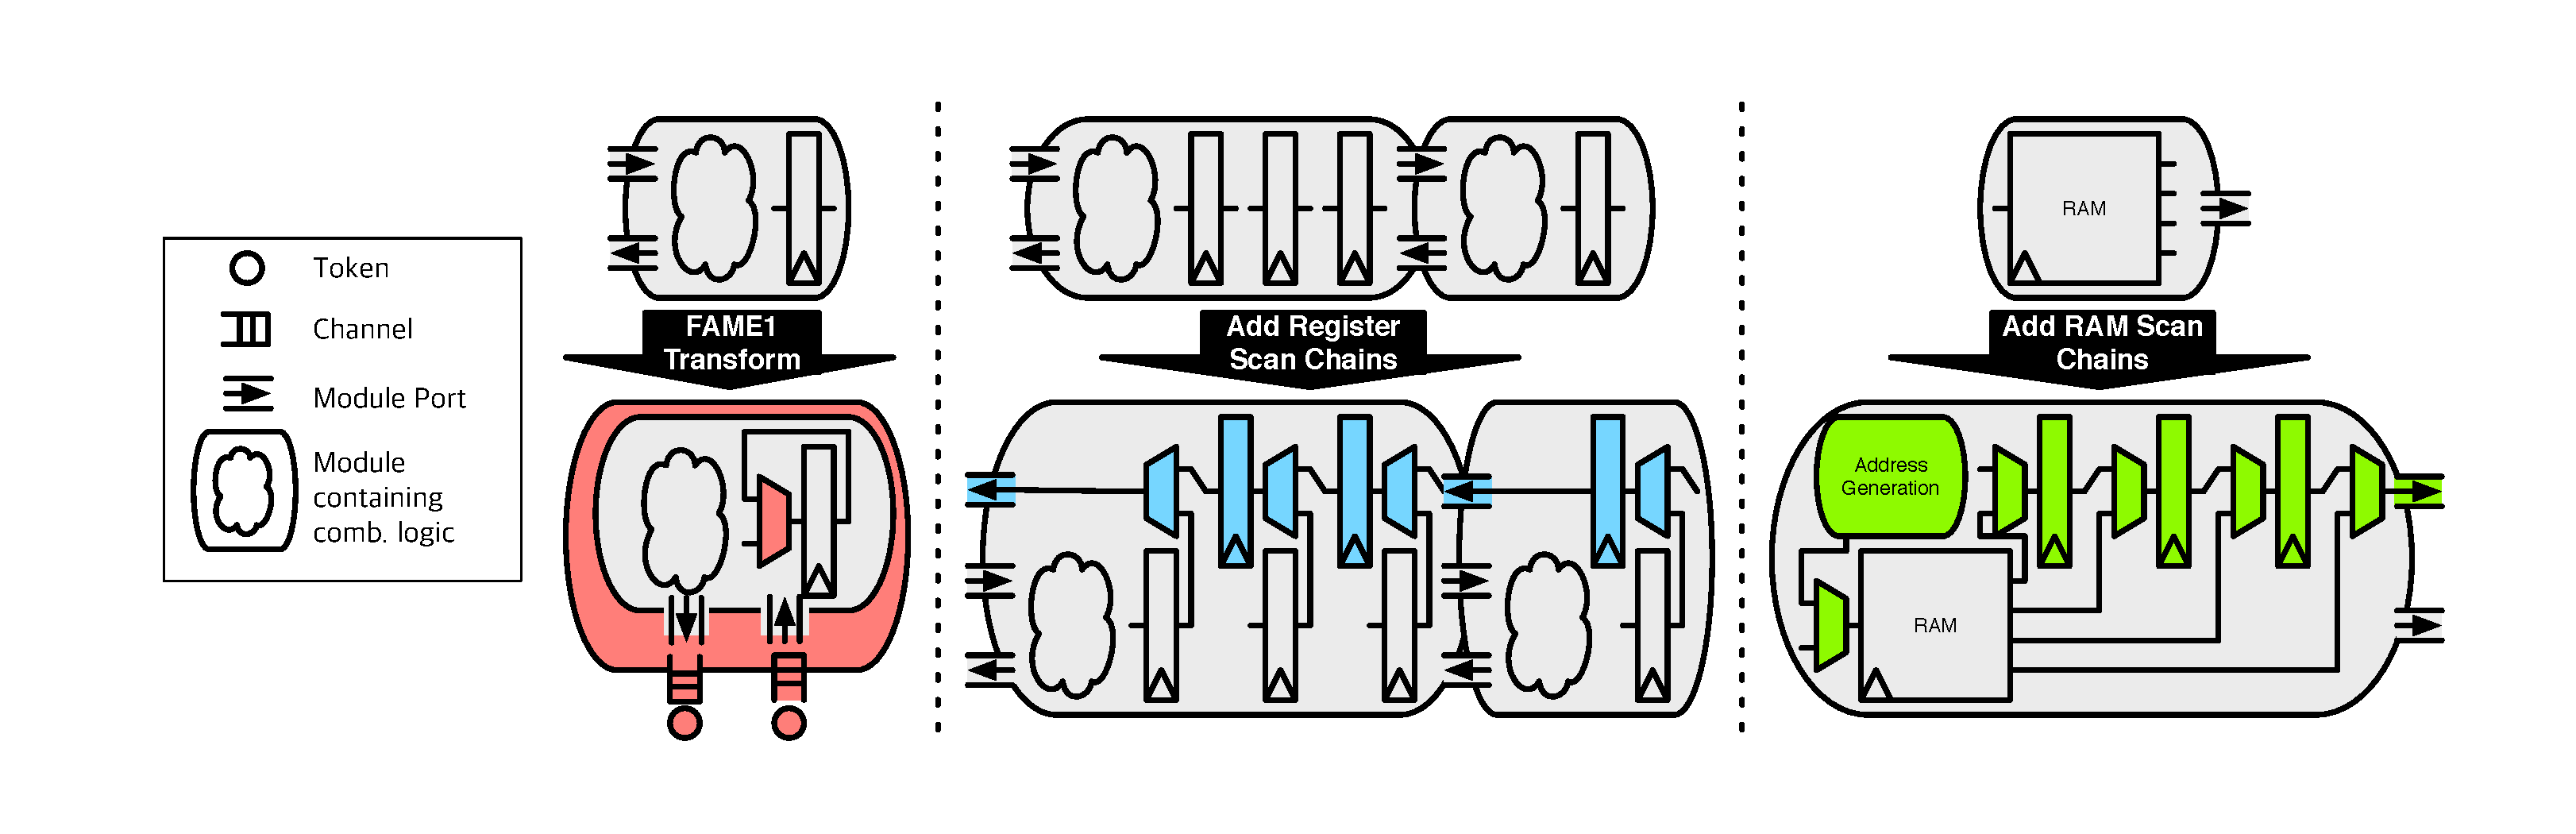
\includegraphics[width=16cm]{figures/midas-passes.pdf}
    \caption{Some passes supported by MIDAS. We often refer to the
    host-decoupling pass as a FAME1 transformation~\cite{fame}.}
	\label{fig:midas-passes}
	\centering
\end{figure}

\subsection{Simulation Mapping}

Once source RTL has been transformed into models, MIDAS generates a
host-agnostic simulation mapping of the SDF. Using Chisel3, MIDAS generates
simulation queues that implement the channels of the SDF. When a channel spans
the boundary of an FPGA, MIDAS generates an \emph{endpoint}, a memory-mapped
queue, whose sister endpoint resides on a different part of the host-platform.
Together, these endpoints implement the simulation channel.  Remaining I/O left
unconnected on transformed-RTL models are bound to the default I/O model, which
acts as an infinite source and or sink of tokens.  When driving an input, the
default I/O model generate tokens with a value set by a memory-mapped register.

During this process, MIDAS also emits \emph{widgets}, memory-mapped modules
that provide simulation utilities but do not simulate target-time (they are not
models). These widgets include scan chain and I/O trace buffer controllers, a
``loadmem" widget used to initialize or dump FPGA-local DRAM, and a master,
that can reset simulation to time zero and regulates the advance of target-time
on the FPGA.

Once all of the simulation components (widgets, models, endpoints. etc...) have
been generated, the simulation interconnect is generated and bound to an AXI4
slave port. All simulation memory-mapped components are managed with MMIO
through this interface. Similarly, components that require FPGA-local DRAM are
bound a single AXI4 master port.\footnote{We recognize this is an unneeded serialization but have only had to support single-channel FPGA-host-memory systems to date.}

\subsection{Platform Mapping}

In attempt to orthogonalize MIDAS from the complexity of FPGA toolchains, MIDAS
requires that the user provide a skeleton project for each FPGA-host type. This
project should expose standard interfaces to its off-chip memory systems and
interconnect, and provide a clock and synchronous reset to drive the
MIDAS-generated RTL.  During platform mapping, MIDAS bridges out the interfaces
exposed in simulation-mapping to the interfaces presented by this project.

Finally, MIDAS emits a ``*Shim.v" that can be compiled into the aforementioned
FPGA project, and a C++ header ``*const.h" that describes the memory map of the
part of the simulation residing on the FPGA.

\section{MIDAS Software Libraries \& User Main}

To control the simulator, the user must build a main and link in the MIDAS C++
libraries, the compiler-generated header and a simulation MMIO driver.  The
MIDAS libraries implement basic commands used to control simulation such as
\emph{step K} and \emph{reset}(these commands will eventually constitute a
``MIDAS API"). Widgets, endpoints, and models instantiated on the FPGA have
their own drivers that extend the basic set of simulation commands. For
example, the default I/O model has \emph{peek}, which reads the value of the
last token sunk through one of its ports, and \emph{poke}, to change the value
of tokens it generates on a specific output port.  All of this functionality is
facilitated with simulation MMIO that must be implemented with a host-platform
specific driver. This simulation MMIO driver supports read and write requests
made by the libraries by tunneling these requests over the interconnect available
on the host.

\section{Target \& Host Machines of this Report}\label{sec:targetandhostmachines}

While MIDAS has preliminary support for other host-platforms, all the
experiments of this report are run on Xilinx ZC706 development boards, which
feature a Zynq XC7Z045 FPGA. These FPGAs have a processing system (PS),
consisting of hardened ARM A9 with 512 MiB of DRAM connected to the
programmable logic(PL), which implements the Kintex-7 fabric architecture with
19.1Mb of BRAM and 350K logic cells. The PS is connected to the PL though a
number of interfaces; we use AXI-GP0, a general purpose 32-bit wide AXI4 master port.
Linux processes running on the PS interact with the PL with MMIO over this
interface. Finally, the PL is connected to a configurable DDR PHY, which on the
ZC706, drives a DDR3 SODIMM (upgraded to 8GiB).

All target designs used in this report are single-core, tethered RISC-V
processors with a single-channel DRAM subsystem.  They all share the MIDAS SDF
shown in figure~\ref{fig:default-target}. This SDF includes: a transformed-RTL
model, sourced with RTL generated by RocketChip, that instantiates the
processor pipeline (Rocket or BOOM), L1 caches, and an uncore containing the
TileLink agent that manages the tether. A software model, which wraps the
RISC-V front-end server (\texttt{riscv-fesvr}) that facilitates tethered boot
and to which console I/O is proxied from the target. And the memory-timing
model instance, which connects to an AXI4 port presented by the processor.
All unconnected I/O of the transformed model, including reset, is bound to the
default I/O model.

\begin{figure}
	\centering
	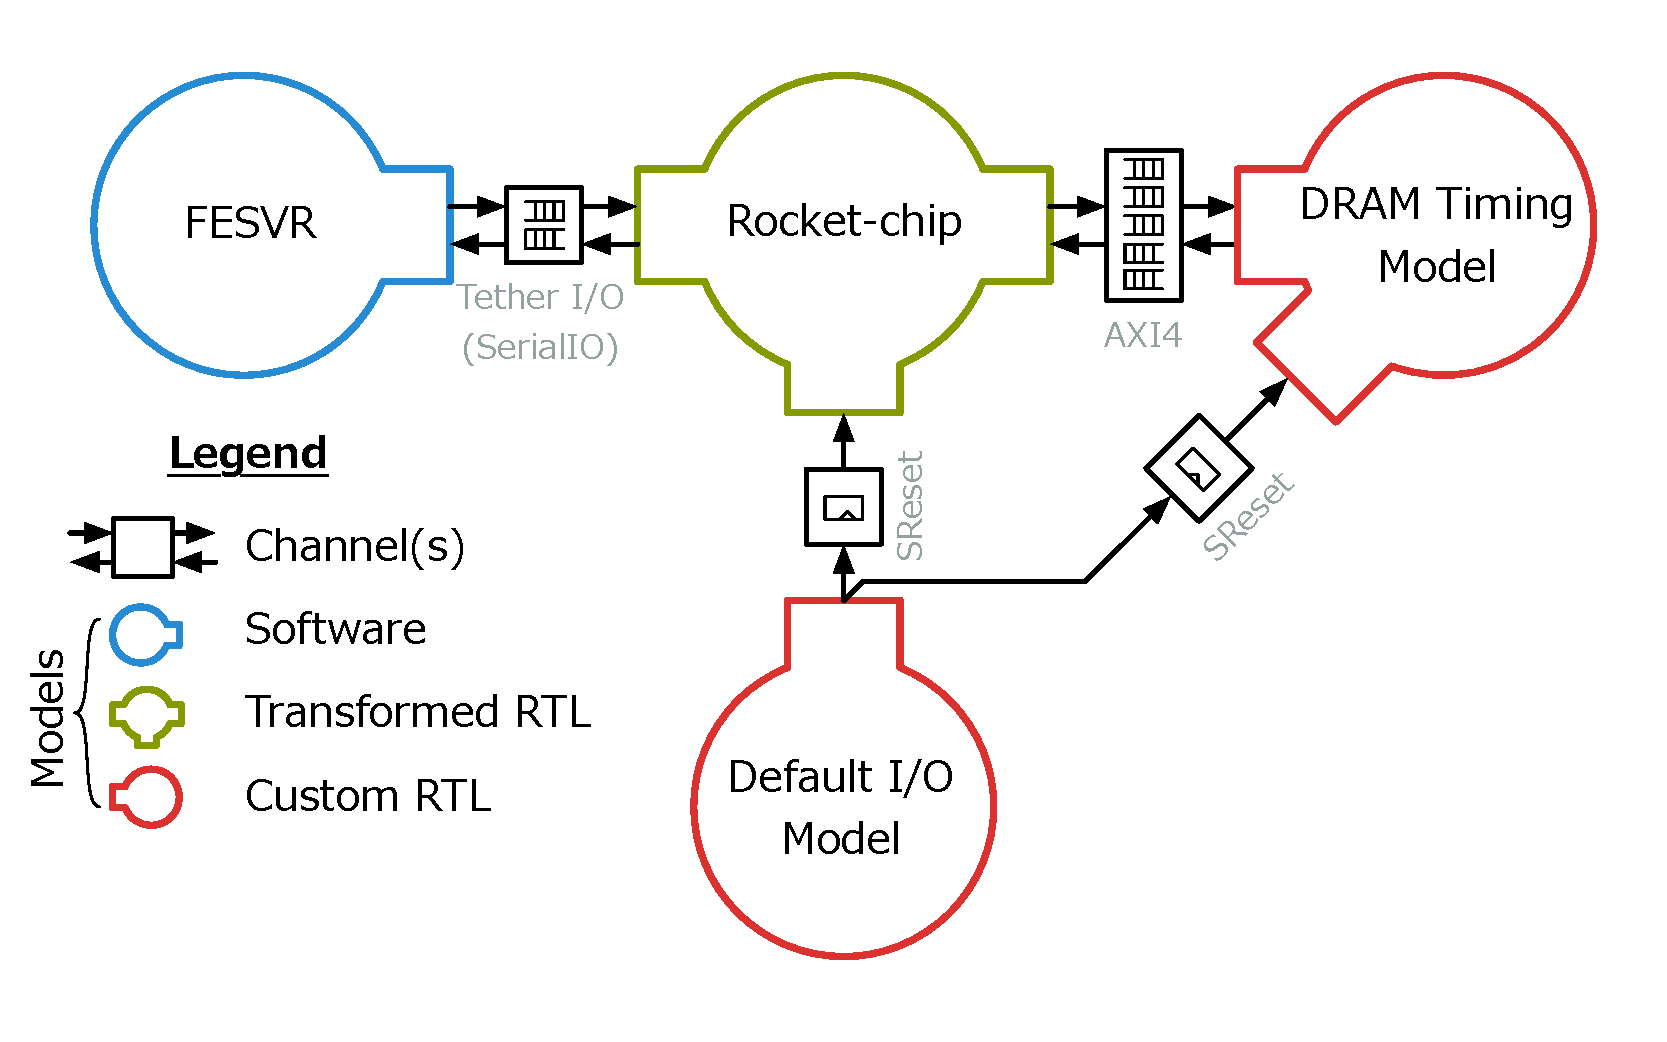
\includegraphics[width=\textwidth]{figures/masters-target.pdf}
    \caption{The MIDAS SDF of the target design used in this report. Channel
    details and initial tokens are omitted for simplicity. Both the tether I/O
    and AXI4 have bidirectional decoupled (ready-valid) target interconnect,
    thus the channels are implemented as sets of queues. SReset channels are pipes with
    a latency of one.}
	\label{fig:default-target}
\end{figure}

\begin{figure}
	\centering
	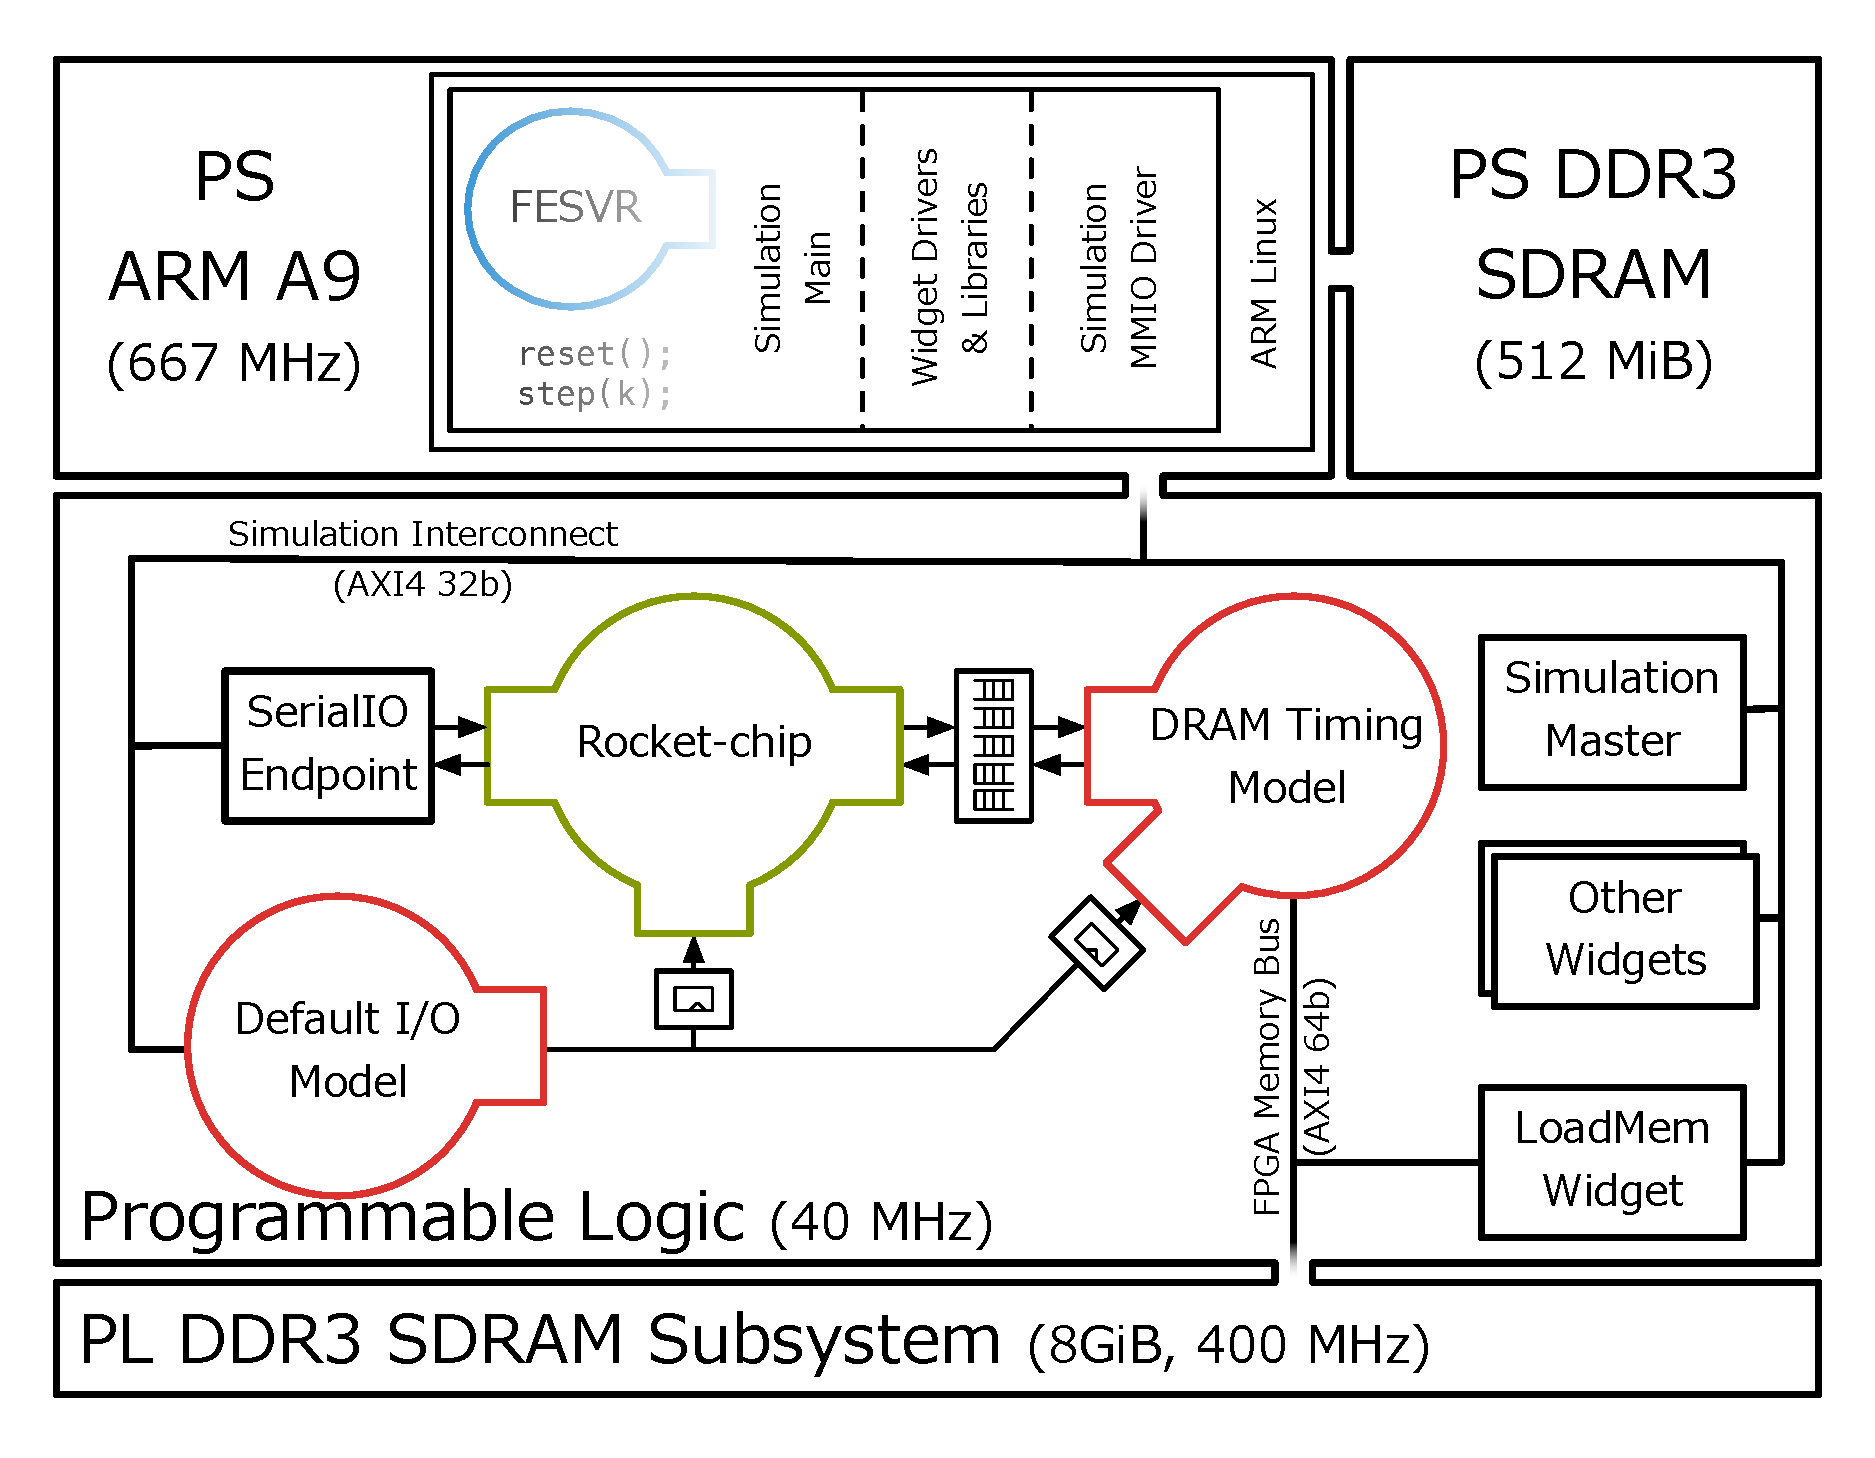
\includegraphics[width=\textwidth]{figures/hosted-masters-target.pdf}
    \caption{The target of figure~\ref{fig:default-target} mapped to the ZC706.}
	\label{fig:hosted-masters-target}
\end{figure}

The simulation is hosted as shown in figure~\ref{fig:hosted-masters-target}.
The simulation main including the \texttt{riscv-fesvr} software model is hosted
on the PS (running in a single linux process) while all other models are hosted
in the PL. The simulation interconnect is bound to the AXI-GP0 port of the PS;
the simulation MMIO driver simply \texttt{mmap}s the memory region bound to that port
into the process' memory space.
